\subsection{Variational Monte Carlo calculations of the Beryllium and Neon atoms}

	We attempt to solve the ground state energy for the Beryllium atom and Neon atom using a Variational Monte Carlo calculation with importance sampling. We have used the trial functions \eqref{eq:BerylliumTrialFunction} for Beryllium and \eqref{eq:NeonTrialFunction} for Neon which uses $\alpha$ and $\beta$ as variational parameters.

	For Beryllium we have the Alpha and Beta values $\alpha=4.0$ and $\beta=0.31$. We use $10^{7}$ cycles and find the energy to be $-14.3902$ au, with a variance of $9.08566 \times 10^{-4}$.
	For Neon, with $10^{6}$ cycles, we get an energy of $-127.875$ au with a variance of $0.0131537$.

	From reseach papers we find the value for energy in the ground state
	of Beryllium to be $-14.667$ au \parencite{Koput_2011_PCCP}  and the value
	for energy in the ground state of Neon to be \(-128.928\) au \parencite{Binkley_1975}.
	In \cref{tab:EnergyAlphaBetaReference} we compare results
	obtained with our Variational Monte Carlo method with results from
	various research papers.

	\subsubsection{Alpha and Beta Values}

		\begin{figure}
			\centering 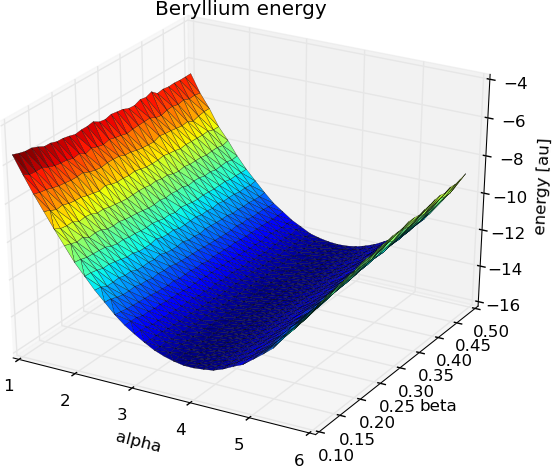
\includegraphics[width=0.45\linewidth]{../figures/Beryllium_alpha_beta_energy}
			\centering 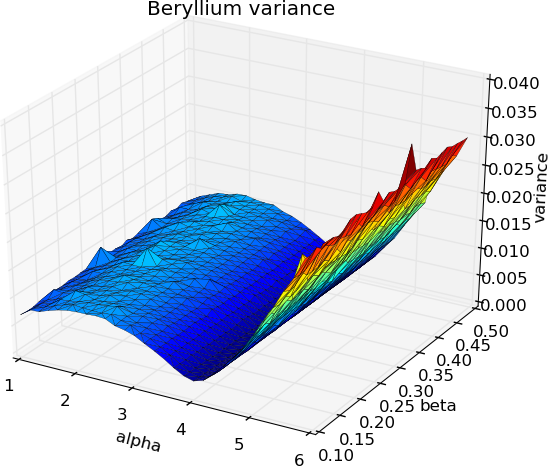
\includegraphics[width=0.45\linewidth]{../figures/Beryllium_alpha_beta_variance}
			\protect\caption{Energy (left) and variance (right) for different Alpha and Beta values for Beryllium, using $10^{6}$ cycles.}
			\label{fig:alpha_beta_comparison_beryllium}
		\end{figure}

		\begin{figure}
			\centering 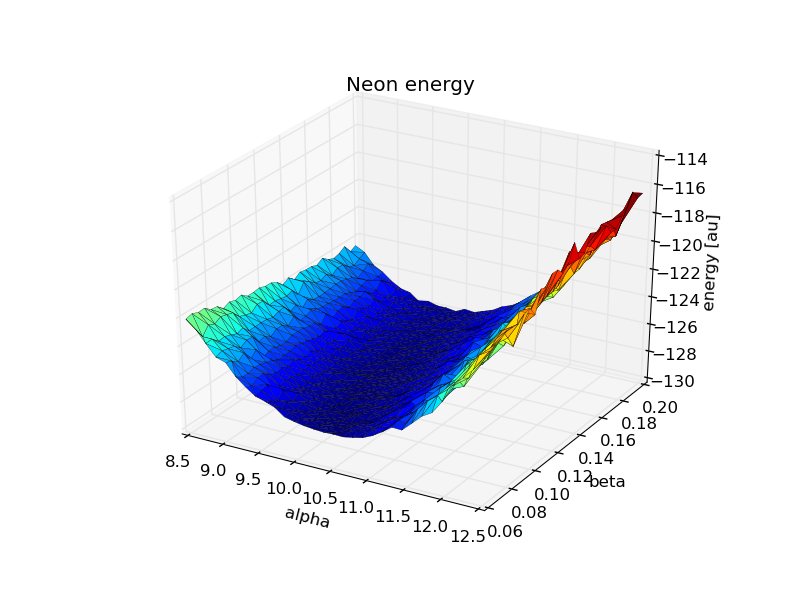
\includegraphics[width=0.45\linewidth]{../figures/Neon_alpha_beta_energy}
			\centering 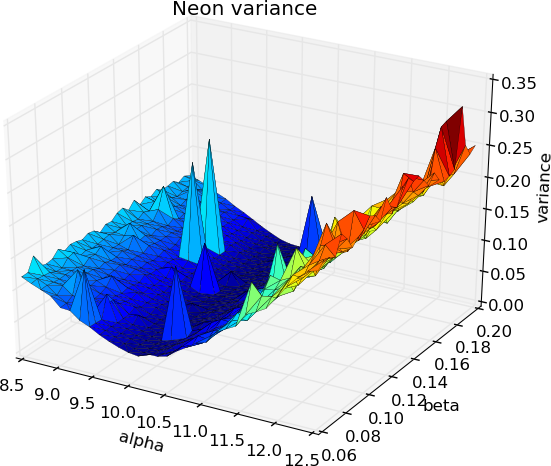
\includegraphics[width=0.45\linewidth]{../figures/Neon_alpha_beta_variance}
			\protect\caption{Energy (left) and variance (right) for different Alpha and Beta values for Neon, using $10^{5}$ cycles.}
			\label{fig:alpha_beta_comparison_neon}
		\end{figure}

		To find optimal Alpha and Beta values for the atoms we run VMC with ranges of different values for \(\alpha\) and \(\beta\). The resulting plots of variance and energy for different combinations are given in figure \ref{fig:alpha_beta_comparison_beryllium} for Beryllium and figure \ref{fig:alpha_beta_comparison_neon} for Neon. The optimal values are shown in table \ref{tab:EnergyAlphaBetaReference}. As VMC runs slowly for Neon, because it has 10 electrons, we were only able to run over the range of Alpha and Beta values with $10^{5}$ cycles. This is reflected in the higher variance, and the spikes in the variance plot.

		\begin{table}
			\center %
			\begin{tabular}{|c|c|c|c|c|c|c|}
				\hline 
				Atom  & $\alpha$ & $\beta$ & Cycles & VMC {[}au{]} & Variance & Reference energy {[}au{]} \tabularnewline
				\hline 
				Helium & $1.843$ & $0.34$ & $10^{8}$ & $-2.89012$ & $7.76888\times10^{-5}$ & $-2.9037$\tabularnewline
				\hline 
				Beryllium  & $4.0$ & $0.31$ & $10^{7}$ & $-14.3902$  & $0.000908566$ & $-14.667$ \tabularnewline
				\hline 
				Neon  & $10.22$ & $0.091$ & $10^{6}$ & $-127.875$ & $0.0131537$ & $-128.928$ \tabularnewline
				\hline 
				H$_2$ & $1.289$* & $0.401$* & $10^7$ & $-1.15828$	& $0.000225$  & $-1.17540$ \tabularnewline
				\hline
				Be$_{2}$ & $3.725$* & $0.246$* & $10^6$ & $ -31.349 $	& $ 0.00756 $  & $-29.339$ \tabularnewline
				\hline
			\end{tabular}\protect\caption{Comparison of energies resulting from our Variational Monte Carlo method with
			energies found in research papers \parencite{Koput_2011_PCCP} \parencite{Binkley_1975}. The values for \(\alpha\) and \( \beta \) where found by doing running Monte Carlo calculation with over a mesh of different \(\alpha\) and \( \beta \) values. The run with the lowest energy gave the \(\alpha\) and \(\beta\) values. For H$_2$ and Be$_2$ we used $\alpha$, $\beta$ values, along withe the benchmark value, from \citet{Ihle_Ledum} and used a nuclei distance of \( 1.40 \) a.u. and \( 4.63\) a.u. respectively. The binding enery found for Be\(_2\) is too low which is caused by a bug in the implementation of the molecule.}
			\label{tab:EnergyAlphaBetaReference} 
		\end{table}


	\subsubsection{Speedup with MPI}
		\begin{table}
			\center
			\begin{tabular}{| c | c| c| c| c|}
				\hline
					\textbf{Num. of processes} &	1	&	2	&	3	&	4
				\\ \hline
				\textbf{Speedup}	&	1.0	&	1.97	&	2.90	&	3.35
				\\	\hline
			\end{tabular}
			\caption{MPI speedup}
			\label{tab:MPI_speedup}
		\end{table}

		\begin{figure}
			\centering 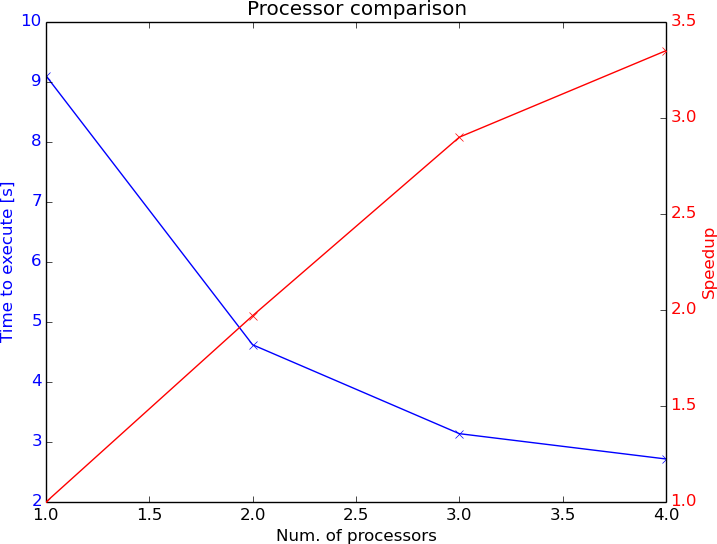
\includegraphics[width=0.45\linewidth]{../figures/processor_number_time_comparison}
			\protect\caption{MPI speedup}
			\label{fig:MPI_speedup}
		\end{figure}

		It is desirable to have a speedup as close as possible to the number of processors used. The speedup measured by our VMC program running 1, 2, 3 and 4 is shown in table \ref{tab:MPI_speedup} and figure \ref{fig:MPI_speedup}. We see that the speedup is good for 2 and 3 processes, but for 4 processes suffers somewhat because it also have to run the OS and other programs.


		\begin{table}
			\center %
			\begin{tabular}{|c|c|c|c|c|c|c|c|}
				\hline 
				Atom  & $\beta$ & Cycles & VMC {[}au{]} & Variance & Ref. energy {[}au{]} & GTO [s] & STO [s] \tabularnewline
				\hline 
				Helium &  $0.34$ & - & - & - & $-2.9037$ & - & - \tabularnewline
				\hline 
				Beryllium  &  $0.109375$ & $7\times 10^{7}$ & $-14.0182$ & $0.00203359$ & $-14.667$ & $48321$ & $4141$ \tabularnewline
				\hline 
				Neon  & $0.091$ & - & - & - & $-128.928$ & - & - \tabularnewline
				\hline 
			\end{tabular}\protect\caption{ Comparison of energies found using bisection method with the refenrence energy \parencite{Koput_2011_PCCP} \parencite{Binkley_1975} and comparison of the time used running the computation with the given number of cycles using GTOs and STOs.}
			\label{tab:AtomsGTO} 
		\end{table}
